\chapter{State of the Art: Optimal path planning for autonomous robots}

\renewcommand{\chaptername}{Chapter}

\section*{Introduction}

The intralogistics sector is undergoing a significant transformation due to the 
integration of digital tools such as connected industries and robotics. The cluttered 
and highly dynamic nature of this environment makes it challenging to successfully 
implement robotic solutions.

The first steps in digitalizing logistic processes with robots involved the use of 
Automated Guided Vehicles (AGVs). First introduced in 1955, AGVs perform tasks like 
material handling. AGVs are managed by top-level software that handles task planning, 
providing the vehicles with intermediate waypoints to navigate from start to end points \cite{R7}. 

However, the decentralized decision-making approach of AGVs makes them 
unresponsive to changes in their environment. For example, AGVs localize themselves 
using specific and precise anchors physically located in their workspace. 

This localization mechanism helps them follow the assigned path. As a result, even 
a simple environmental change of the dispositionsrequires an update of the measurements 
and maps on  which the planning is based. Another example is that an AGV is unable to plan and 
execute a solution if it encounters an obstacle on its way to the goal or it arrives at a shifted 
destination. In such cases, 
the AGV’s reaction is to stop and wait for top-level instructions \cite{R8}. This behavior 
decreases productivity and disrupts the planned sequence of tasks until an intervention is managed.

To overcome these disadvantages of AGVs, Autonomous Mobile Robots (AMRs) were introduced. 
AMRs are equipped with a decentralized control system, enhanced perception of their 
surroundings through more complex hardware, and advanced software to manage and integrate 
these hardware additions (Figure \Ref{AMR-VS-AGV}).

\begin{figure}[H]
    \begin{center}
       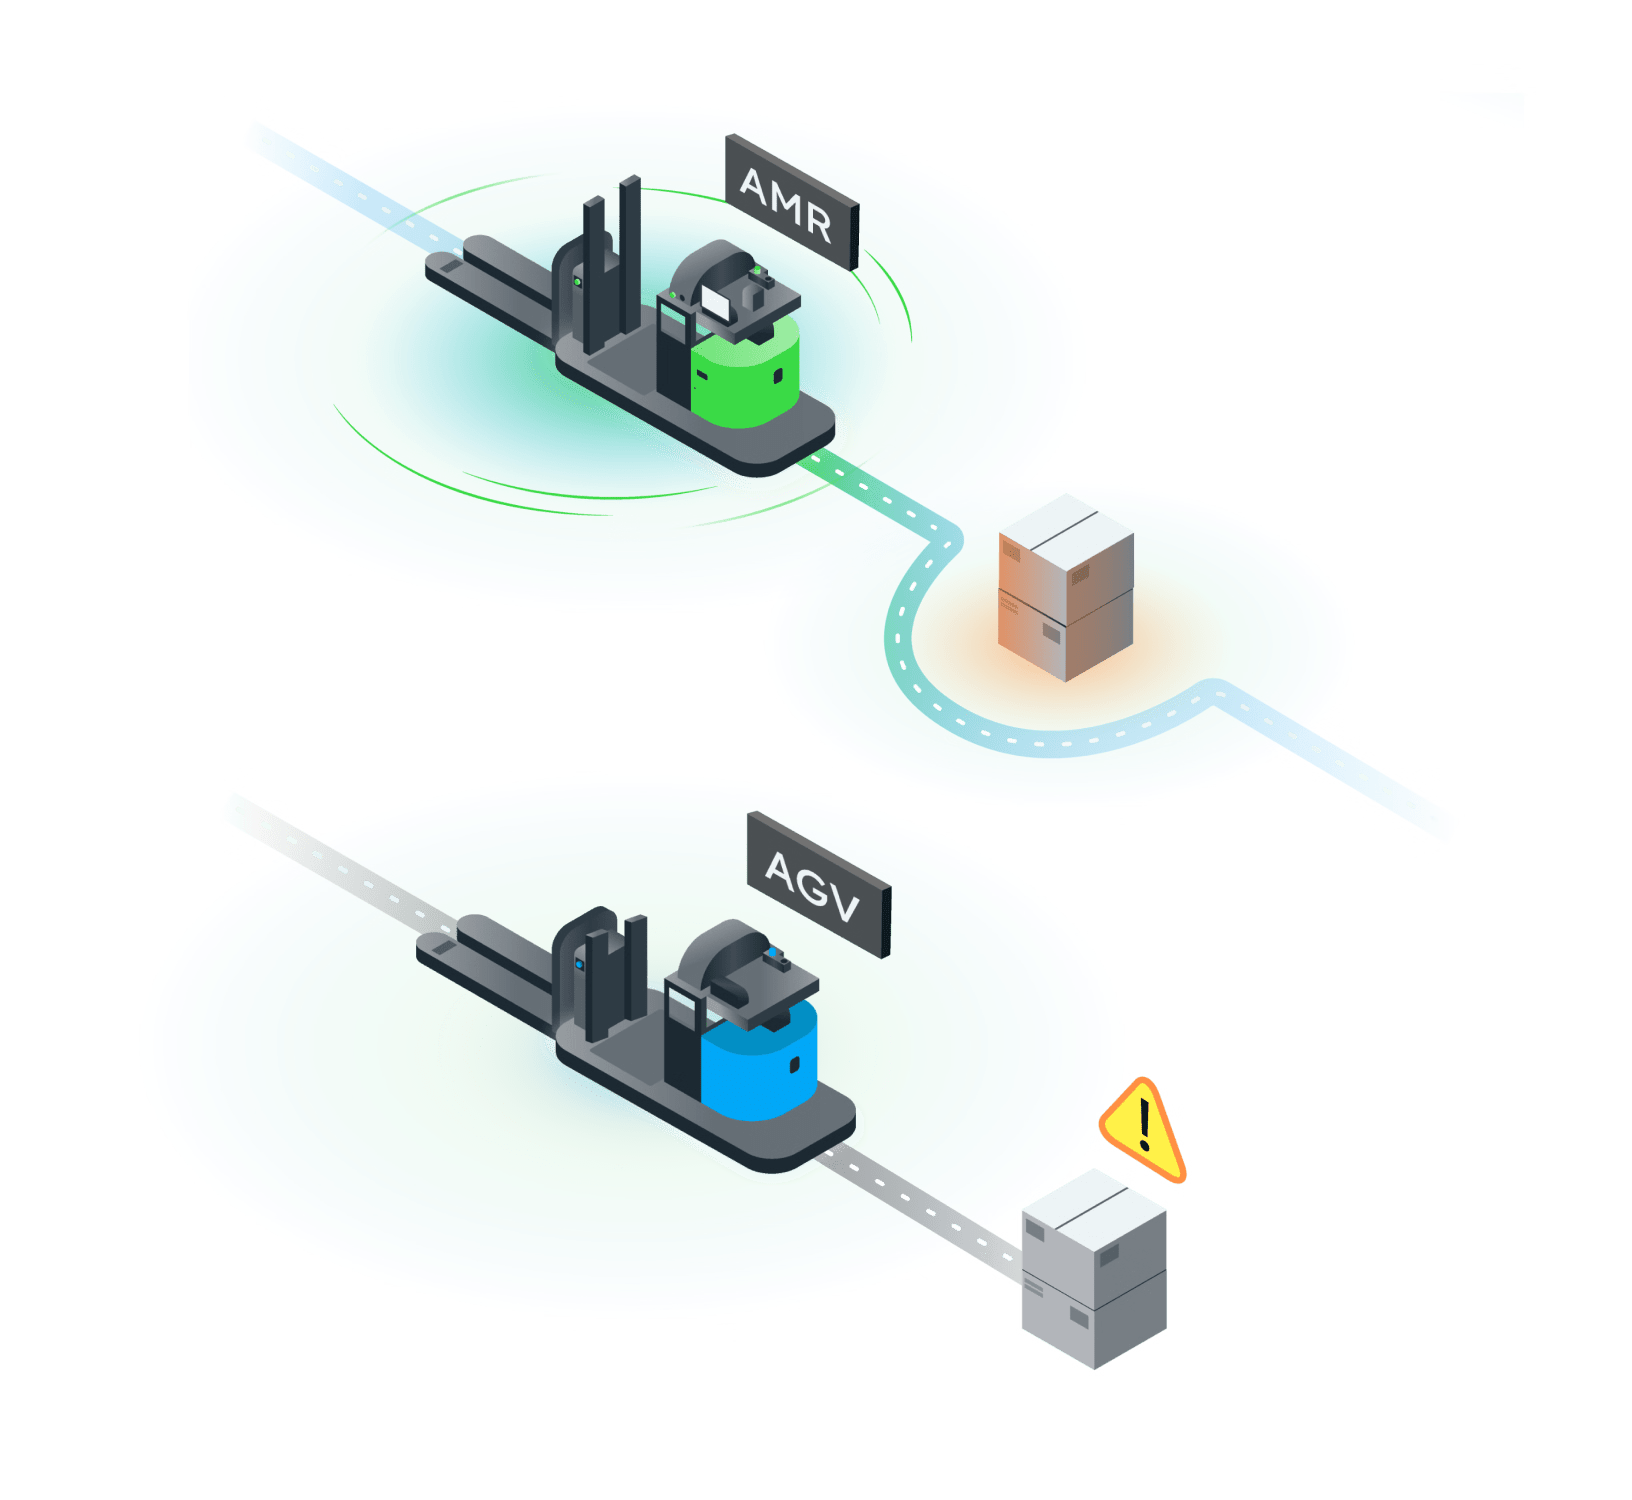
\includegraphics[width=4in]{images/Chap1/AMR-VS-AGV.png}\\
       \caption{AMR and AGV behaviors at presence of an obstacle \cite{R9}}
       \label{AMR-VS-AGV}
       \end{center}
\end{figure}

In addition, they grant a fast integration into new environments due to smart perception 
and recognition technologies. AMRs use this data as input to smart algorithms that 
enable it to plan its missions, navigate to its destination, avoid collisions, and 
execute missions all while collaborating with humans in the working space. The 
Autonomous vehicles do not require an automation expert or a roboticist’s presence to 
be configured or to deal with complex situations. It is able to solve such situations 
individually due to the scalable software that it has on board.

On the one hand, this evolution enables AMRs to navigate more dynamically and adaptively 
within intralogistics environments, improving overall efficiency and responsiveness. 
On the other hand, the level of flexibility that AMRs brings important safety and 
efficiency considerations \cite{R7}.

One of the main challenges is developing the navigation mechanisms. In a logistics 
environment, it is crucial to comply with the nature of the workspace. The AMR should 
recognize the location of materials to be handled and be able to navigate to and from 
those locations to next missions. Building a flexible and efficient solution requires a 
deep understanding of the situations and special cases that the vehicle may encounter 
and a study about how to create scalable solutions for such events.  

Before diving into the methodologies and technologies used to address this thesis’ 
topic, it is relevant to examine the related works. This research will serve later in 
the thesis as a guiding outline. Literature helps to investigate the level of progress that 
other researchers reached in similar topics, prevents re-invention of existing concepts, 
and pushes to ethically exploit the developed technologies. For this thesis, it is 
important to deeply examine the research papers and scientific resources to build a 
solid foundation of knowledge, identify the gaps in some studies, and propose novel 
solutions.  

In this context, this state-of-the-art report, delves 
into pathplanning and near-field path planning for mobile robots 
in general and for intralogistics AMRs specifically. Then, it examines possible 
solutions for path creation and generation. Afterwards, 
it studies the decision-making science approaches that can be used to evaluate and 
optimize path suggestions. Finally, this chapter 
outlines the methodology to be followed throughout this scientific work(Figure \ref{mindmap}).

\begin{figure}[H]
    \begin{center}
       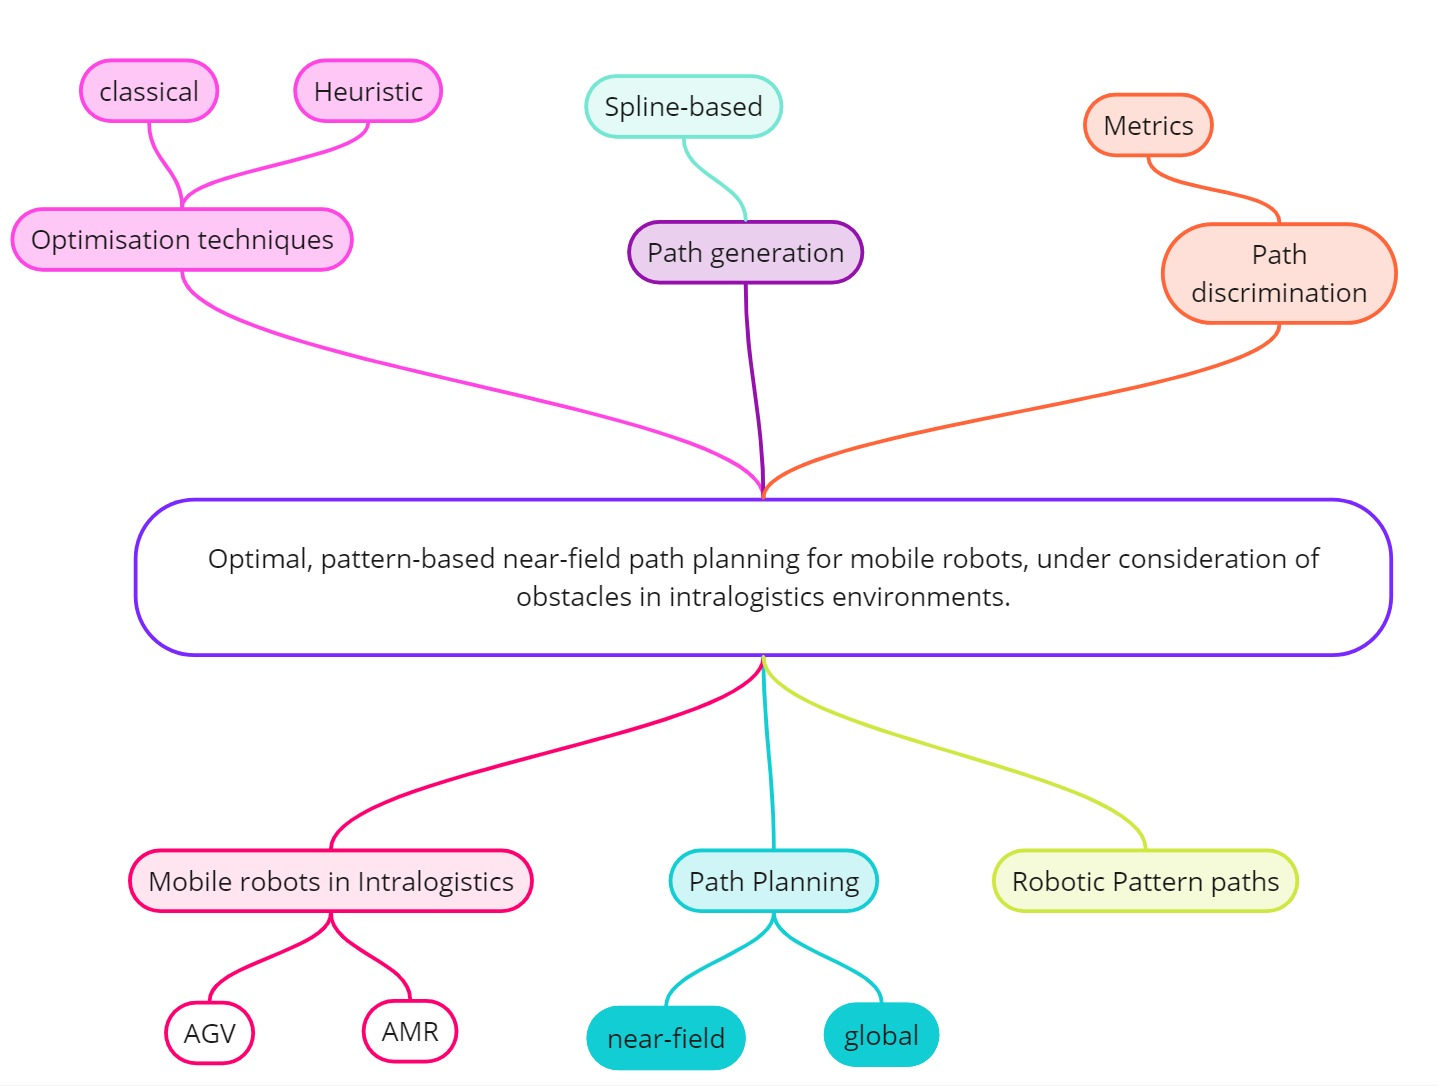
\includegraphics[width=5in]{images/Chap1/Fig1.jpg}\\
       \caption{Mind map of the key topics}
       \label{mindmap}
       \end{center}
\end{figure}

\newpage
\section{Path Planning}

\subsection{Path Planning for autonomous robots: Opportunities and challenges}

Path planning for mobile robots involves creating and generating efficient routes 
for the robot to travel from a starting position (A) to a target position (B), 
ensuring minimal time and travel distance while avoiding collisions with nearby objects.

In complex environments, it is challenging for robots to move randomly and fulfill 
their missions. However, with appropriate input from various sensors, such as laser 
scanners, cameras, and LiDAR, robots can perceive their surroundings and plan 
accordingly. This application is especially relevant in dynamic intralogistics 
environments where operators and employees are moving around; boxes and pallets are 
being transported or stocked; and in warehouses with multiple layers of shelves that 
must be handled safely and carefully. Autonomous robots, as the name suggests, are 
standalone systems that must compile and process such input and generate, with the 
support of powerful algorithms, efficient paths. Path planning serves as the crucial 
link between the robot’s sensor input and its motion control \cite{R10}.

Literature and scientific studies differentiate between two main types of path planning: 
global and local path planning. Global planning involves finding an optimal path from 
the start to the target position based on sensor input within a known, static environment, 
whereas local planning focuses on real-time obstacle avoidance, typically used while 
moving to avoid dynamic obstacles \cite{R11}.

Efficient path planning is essential for ensuring the safe handling of objects in the environment. 
In intralogistics, the materials being handled—whether goods, manufacturing systems, storage 
shelves, or other vehicles—are valuable and must be treated with care. Moreover, safety is a 
critical concern, especially when human safety and protection are involved. To pass quality 
tests, autonomous forklifts must meet personal safety requirements. These requirements include, 
but are not limited to, maintaining a safe distance from both static and dynamic objects and 
people, as well as detecting surroundings at any height and time. By following an efficient 
path, overall productivity increases since operations are repeated many times throughout the 
day. An efficient path optimizes both length and smoothness, thereby reducing travel time. 
Additionally, efficient path planning conserves the truck's energy, reducing the frequency of recharging.

However, developing efficient paths comes with certain limitations. Several studies have compared 
various planners, analyzing the advantages and drawbacks of each. One common drawback is excessive 
computational time: if the algorithm takes too long to process (in the range of seconds), it 
leads to long latencies and vehicle stops. While experts might understand this behavior, clients 
may find it unacceptable, leading to doubts about the vehicle's efficiency or even disinterest in the product.

In very crowded or complex areas, some planners may struggle to generate a viable path, which 
could cause the vehicle to fail in navigating such environments, thus limiting its usefulness 
in real-world scenarios. In these specific cases, some path planning algorithms perform better 
than others. Therefore, it may be beneficial to equip the autonomous vehicle with more than one 
approach for solving such situations (in Section ... the OMPL: Open Motion Planning Library is 
presented as one of the available and most recent tools in RACK). Additionally, embedded PCs, 
often used in these systems, have limited processing power and must handle large amounts of data 
quickly. Achieving short computational times can be challenging, potentially impacting the vehicle's performance.

Furthermore, sensors can produce noise or shadows, leading to uncertainty in the data about the 
terrain. This uncertainty can cause the planner to make errors, affecting the vehicle’s ability 
to navigate accurately and safely \cite{R12}.

\subsection*{Path Planning}
\subsubsection{Global Path Planning}

At the beginning of the research phase for this thesis, it was important to look at the available types 
of path planning methods. Science generally distinguishes between three general approaches of Global 
Path Planning all having the same aim to plan the path from a start to a goal position within a pre-mapped 
environment:  grid-based methods, sampling-based methods, and artificial intelligence-based methods \cite{R13}. 

Grid-based methods involve discretizing the environment into a grid of cells, where each cell represents 
a small, discrete part of the space. Then, the algorithm visits the grids to decide which cells will 
be used for the path based on the occupancy or cost and calculates the fitness function from start to 
the reached point in A* algorithm for example or from the reached point to the destination for Dijkstra 
Algorithm. While this method seems easy to understand and quite simple to implement, it is 
computationally intensive because of the number of grids to evaluate and the repetitiveness 
and constrained in direction (Figure \Ref{direction possibilities}) 

Sampling-based algorithms do not discretize the entire environment into a grid but instead randomly sample 
the space to construct a path: the samples are distributed in a manner that they avoid the obstacles 
and serve as a roadmap for to create a start-to-end path \cite{R15}. The exact approach to transform the 
roadmap into a continuous path depends on the algorithm like PRM or RRT. 

Sampling-based algorithms present advantages like handling big environments and complex situations, 
however, they can also be computationally intensive and demanding in such situations. 
Figure 2 shows the difference in the resulting optimal path in a cluttered environment where with 
1 core the algorithm successfully finds a feasible path, and, as the cores double, the computed path 
improves its quality as the search tree expands.  

\begin{figure}[H]
    \begin{center}
       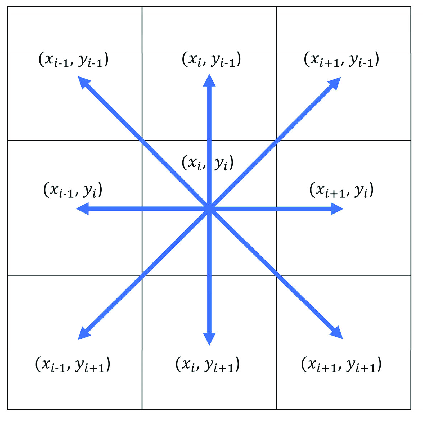
\includegraphics[width=3in]{images/Chap1/8dirs_pathPlan.png}\\
       \caption{8 direction possibilities to move from the current cell to the next cell \cite{R14}}
       \label{direction possibilities}
       \end{center}
\end{figure}

\begin{figure}[H]
    \begin{center}
       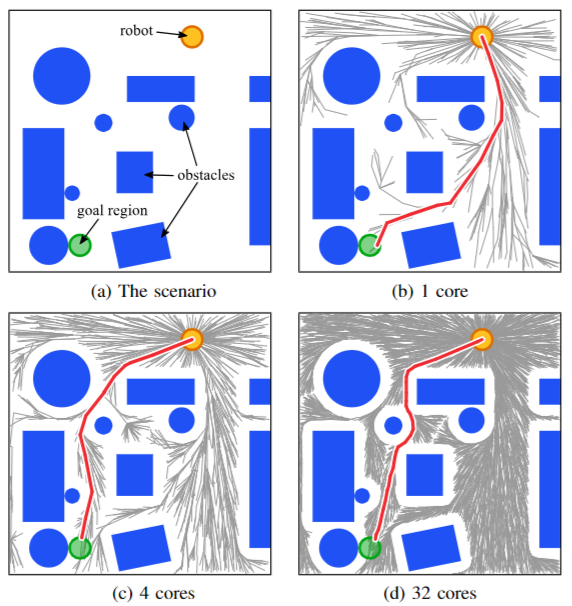
\includegraphics[width=4in]{images/Chap1/sampling-based.png}\\
       \caption{8 direction possibilities to move from the current cell to the next cell \cite{R16}}
       \label{sampling-based}
       \end{center}
\end{figure}

As for artificial intelligence-based methods, also known as heuristic and metheuristic approaches, 
leverage the use of neural networks, machine learning and deep learning, and evolutionary algorithms. 
These methods learn from experience, adapt to changes, and optimize paths in complex environments. 
They are good at handling dynamic and unpredictable scenarios, making them suitable for tasks like 
autonomous driving, robot navigation, and logistics. 

To start with, Neural networks (NN) are inspired from the biological harmonious connection of the brain neurons
that gives it the ability to process big amounts of data and generate ideas and decisions and solve problems. 
The NN is built in a way that enables it to get its input in a form of data and process it by learning, improving 
and adjusting the output to the desired results. NN are able to perform Parallel processing: the information is 
transmitted in two
directions to the neuron in the case of Recurrent Neural Networks (RNN) that allows for learning fron current and 
past inputs to the NN. This approach improves the computation time and overall performance. 
The NN is then able to process complex solutions and create paths for difficult environments. 
It is well suited for unpredictable situations as it is built to adapt to the available input and the desired output.
However, it presents a practicality challenge. Althugh the performance an results can be impressive, yet, in a 
real-time context, 
it is hard to rely on solutions that require extensive computational efforts and need long durations to 
process solutions. In addition, the number of neurons and layers have to be scalable and depends closely on the 
level of complexity that the vehicle is to deal with \cite{R12}. 

Fuzzy Logic (FL), on the other hand, is a way of thinking that mimics how humans make decisions, especially when things are unclear 
or uncertain. Instead of working with exact numbers, it uses "fuzzy" terms like "good", "average" or "bad" to make 
decisions. Input numbers are clustered following the fuzzy sets or intervals and assigned a value using membership 
functions. Later the values are interfered and defuzzified to genearte the ouput as a command value. 
In robotics and path planning, FL helps robots navigate by allowing them to handle uncertain situations, 
like avoiding obstacles or finding the best route, even when the environment is not fully known. Instead of needing 
exact data, the robot can employ fuzzy terms like "close" or "far" to understand its surroundings. For example, if an 
obstacle is "somewhat close," the robot can smoothly adjust its path to avoid it. FL also helps the robot choose the best 
route by weighing various factors like distance and safety, even when the information is not perfect. This makes the 
robot better at handling unpredictable environments and making flexible and optimal decisions.
However, one 
disadvantage is that it can be tricky to create the right rules for the robot to follow, and the system can become 
complicated as more rules are added. It may present a scalability problem because in unpredictable and dynamic environments
it is not simple to decide about fixed fuzzy sets that would be practical in all of the cases \cite{R12}.

While Neural Networks and Fuzzy Logic offer powerful approaches for handling uncertainty and complex decision-making, 
another key area in artificial intelligence for path planning is the use of meta-heuristic algorithms.
Meta-Heuristoc algorithms are inspired from biological and natural processes for evolution and survival. 
Unlike NN and FL, that rely on data as input to generate decisions, meta-heuristic algorithms explore the solution
space by evolving random solutions for the problem and optimizing them by rounds until a stopping criterion or set
of criteria is satisfied (see more in section ...: Optimization Algorithms).
Approaches like Genetic Algorithms (GA) have been used for path planning by Ahmed Elshamli et al. \cite{R17}. The The robusteness of their 
solution is the adaption of the solution to dynamic environments. They evolve their GA using variable size chromosomes, where each node 
represents a waypoint of the path, then they measure the quality of each path using an evaluation function. A modified Genetic Approach is then 
applied to each population: Crossover, mutation, \textbf{Repair} infeasible paths, \textbf{Shorten}, then \textbf{Smoothen} 
feasible paths while dynamically checking for new obstacles.
The approach is tested in static and dynamic environments and has achieved proven efficiency when it comes 
to local optima challenges and survivig the best elements of the population. While the use of the GA itself is robust
and successful, it can be challenging to recreate the algorithm and to add the improvements. In addition, the tests
the ran are limited to a simple simulation with unrealistic situations and obstacle setting as displayed in 
figure \Ref{R17 test scenarios}. 

\begin{figure}[h!]
    \centering
    \begin{minipage}{0.30\textwidth}
        \centering
        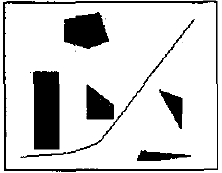
\includegraphics[width=\linewidth]{images/Chap1/R17_simple.png} % Replace with your figure
        \caption{Simple obstacle environment       }
        \label{Simple obstacle environment}
    \end{minipage}
    \begin{minipage}{0.30\textwidth}
        \centering
        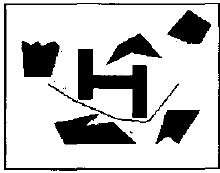
\includegraphics[width=\linewidth]{images/Chap1/R17_intermediate.png} % Replace with your figure
        \caption{Intermediate obstacle environment}
        \label{Intermediate obstacle environment}
    \end{minipage}
    \begin{minipage}{0.30\textwidth}
        \centering
        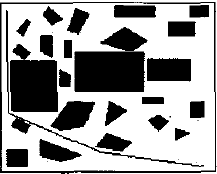
\includegraphics[width=\linewidth]{images/Chap1/R17_complex.png} % Replace with your figure
        \caption{Complex obstacle environment}
        \label{Complex obstacle environment}
    \end{minipage}
    \caption{GA Test scenarios \cite{R17}}
    \label{R17 test scenarios}
\end{figure}

\subsubsection {Local Path Planning}
Local path planning is a process used by robots to make real-time decisions about how to move 
safely and efficiently in their surroundings. Unlike global path planning, which focuses on 
finding the best overall route from a starting point to a destination based on astatic map, local path 
planning deals with navigating the environment directly around the robot while considering real-time
data input from sensors \cite{R18}. This involves quickly responding 
to obstacles that suddenly appear or changes in the terrain, ensuring the robot can continue moving 
without collisions.

Local path planning is crucial for the safe and effective operation of robots, especially in 
environments where situations can change in a fast manner. For example, in busy spaces with moving people 
or vehicles, a robot needs to be able to make quick adjustments to avoid accidents. This type of 
planning allows the robot to react immediately to new information, making it essential for applications 
where unpredictability and quick responses are vital, such as in autonomous vehicles or service robots.
Local path planning is crucial for the safe and effective operation of robots, especially in 
environments where conditions can change rapidly. For example, in busy spaces like warehouses 
with moving people or vehicles, a robot needs to be able to make quick adjustments to avoid accidents. 
This type of planning allows the robot to react immediately to new information, making it essential for 
applications where unpredictability and quick responses are vital, such as in autonomous vehicles 
or service robots.

Common Techniques involve Reactive methods which are approaches in local path planning that focus on real-time
obstacle avoidance and online adjustements on the path that are processed while the robot is navigating.
Techniques like the Vector Field Histogram (VFH), 
Dynamic Window Approach (DWA), and Potential Fields are commonly used.

\subsubsection {Hybrid Path Planning}


In \cite{R19}, Liu et al. worked used Djikstra ALgorithm for Global path planning and 
the DWA as the local path planner for sudden unkown obstacles that could 
appear for smart cars while following the global path.
It works by evaluating different possible movements the robot could make within a short time frame 
and choosing the one that avoids obstacles while also moving towards the goal. The "window" refers 
to a limited set of possible velocities of the velocity space the robot can use based on its current 
speed and capabilities. Figure \Ref{flowchart of the DWA} details the flowchart of the DWA. 

The combined algorithms were tested on 3 spaces with 3 stages of environment complexity ranging from 
simple to complex. The tests showed that the hybrid path planning approach was efficient for navigating the 
robot and avoiding collisions. However, the tests were effected with dynamic obstacles only inside the simulation.


Sensor-based approaches, on the other hand, rely on data collected by the robot's sensors, such as LIDAR, 
sonar, or cameras, to make decisions about where to go next. These sensors help the robot create a map of 
its surroundings, which can then be used to identify obstacles and safe paths. Occupancy grids and Point 
cloud processing are techniques used to interpret the sensor data and guide the 
robot's movements. This approach allows the robot to have a detailed understanding of its immediate 
environment, making it more capable of avoiding obstacles and navigating complex spaces.

\begin{figure}[H]
    \begin{center}
        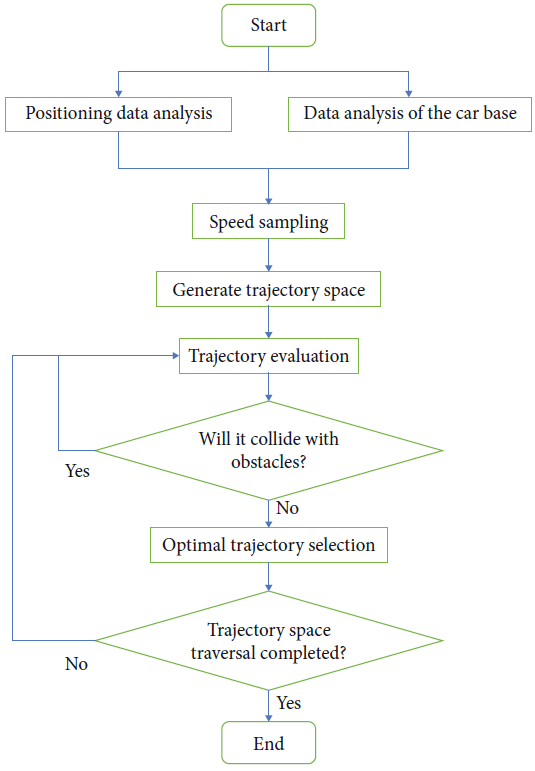
\includegraphics[width=3in]{images/Chap1/DWA_flowchart.png}\\
        \caption{Flowchart of the DWA \cite{R19}}
        \label{flowchart of the DWA}
        \end{center}
\end{figure}



\subsection {PathOMPL}
current solution : path OMPL + BFMT + Reeds-Shepp
there has to be multiple solutions 
ompl is not station specific

The Open Motion Planning Library also known as OMPL, 
\subsection{conclusion}


\section{Spline based Paths}
\section{Metrics}
\section{Optimization Techniques}








